\documentclass[12pt]{article}
\setlength{\parskip}{\baselineskip}%
\setlength{\parindent}{0pt}%
\usepackage{amsmath}
\usepackage{amssymb}
\usepackage{graphicx}
\graphicspath{ {images/} }
\usepackage{hyperref}
\usepackage[shortlabels]{enumitem}
%\usepackage{tikz}
%\usetikzlibrary{trees}
\usepackage[top=1in, bottom=0.75in, left=0.75in, right=0.75in]{geometry}
\newcommand*{\Scale}[2][4]{\scalebox{#1}{\ensuremath{#2}}}%
\usepackage{listings}

\begin{document}

\title{\vspace{-5ex}Math 793: Cramer's Rule}
\author{by Gary Dalton}
\date{\vspace{-3ex}due February 23, 2021}
\maketitle

\section{Introduction}
The goal of this project is to solve a system of linear equations using Cramer's rule instead of using the current standard methodologies.

We will consider linear equations in the form of $Ax=b$, where $A$ is a non-singular $n\times n$ matrix, $b$ is a $n\times 1$ unknown vector, and $b$ is a given $n\times 1$ vector. Cramer's rules states that
\begin{align*}
	x_i = \frac{\det(A_i(b))}{\det(A)}, i=1,2,\cdots,n
\end{align*}
where $A_i(b)$ denotes the matrix $A$ with its ith column replaced by $b$.

The standard method of computing the determinant by recursion of minors is not an efficient computation algorithm. In fact, its complexity is of $O(N!)$, which makes it useless for real world problems. Instead, methods are used to row reduce the matrix to obtain upper and lower triangular matrices and then compute the determinate from those.

This document may contain code examples but most code examples are included by reference to the accompanying Jupyter notebook, at \url{https://github.com/gary-dalton/math793/blob/main/notebooks/Introduction.ipynb}.

\subsection{Example}
Consider the following system of equations:
\begin{align*}
	a_{1,1}x_1 + a_{1,2}x_2 + a_{1,3}x_3 = b_1 \\
	a_{2,1}x_1 + a_{2,2}x_2 + a_{2,3}x_3 = b_2 \\
	a_{3,1}x_1 + a_{3,2}x_2 + a_{3,3}x_3 = b_3
\end{align*}
With
\begin{align*}
	&A = \begin{bmatrix}
		a_{1,1} & a_{1,2} & a_{1,3} \\
		a_{2,1} & a_{2,2} & a_{2,3} \\
		a_{3,1} & a_{3,2} & a_{3,3}
	\end{bmatrix}, &
	&x = \begin{bmatrix}x_1 \\	x_2 \\	x_3	\end{bmatrix}, & 
	b = \begin{bmatrix} b_1 \\	b_2 \\	b_3	\end{bmatrix}&
\end{align*}
Then
\begin{align*}
	x_1 &= \frac{\det\begin{bmatrix}
			b_1 & a_{1,2} & a_{1,3} \\
			b_2 & a_{2,2} & a_{2,3} \\
			b_3 & a_{3,2} & a_{3,3}
		\end{bmatrix}
	}{\det(A)}, &
	x_2 = \frac{\det\begin{bmatrix}
			a_{1,1} & b_1 & a_{1,3} \\
			a_{2,1} & b_2 & a_{2,3} \\
			a_{3,1} & b_3 & a_{3,3}
		\end{bmatrix}
	}{\det(A)}, & &
	x_3 = \frac{\det\begin{bmatrix}
			a_{1,1} & a_{1,2} & b_1 \\
			a_{2,1} & a_{2,2} & b_2 \\
			a_{3,1} & a_{3,2} & b_3
		\end{bmatrix}
	}{\det(A)}&
\end{align*}


\section{Current Approaches}
Current technology with python to solve a system of linear equations uses \textit{scipy.linalg.solve}. This in turn uses routines from LAPACK, "The generic, symmetric, Hermitian and positive definite solutions are obtained via calling ?GESV, ?SYSV, ?HESV, and ?POSV routines of LAPACK respectively."

There are specialized solutions for known special matrices, but we are most interested in the generic solver. From the documentation of ?GESV, we have, 
\begin{quote}
?GESV computes the solution to a real system of linear equations
\begin{align*}
	A * X = B
\end{align*}
where A is an N-by-N matrix and X and B are N-by-NRHS matrices.

The LU decomposition with partial pivoting and row interchanges is
used to factor A as
\begin{align*}
	A = P * L * U
\end{align*}
where P is a permutation matrix, L is unit lower triangular, and U is
upper triangular.  The factored form of A is then used to solve the
system of equations $A * X = B$.
\end{quote}
The complexity of the ?GESV algorithm is indicated as $O(.67N^3)$. This is obtained from table 3.13 in \url{https://www.netlib.org/lapack/lug/node71.html}.
\\\\
\textbf{Note}: The relationship between Scipy and Numpy is close. Generally the functions are equivalent.

\subsection{Solution to System of Equations}
The soltuion to a system of equations is found using forward and backward substitution.
\begin{align*}
	Ax &= b \\
	LUx &= b \\
	Ly &= b \\
	Ux &=y
\end{align*}
Where $Ly=b$ is solved using forward substitution and $Ux=y$ is solved using backward substitution. The great advantage of this approach is that the LU decompistion and forward substituion are performed once to find all of the solutions. This adds a complexity to the algoritm of no more than $O(n^2)$.

\subsection{Determinant}
Determinants of triangular matrices are easily calculated as the product of the diagonal entries. Thus $\det(L) =1$ and $\det(U)$ is easily calculated by $O(n)$ operations. Since P is a permutation matrix, its determinant is trivial to calculate using the method of minors and is of order $O(n)$. $det(P)$ equals either $1$ or $-1$. So that we have:
\begin{align*}
	\det(A) = \det(P) * \det(U)
\end{align*}
This is the method used by both numpy and scipy to calculate a determinant.


\subsection{Cramer's Rule and LU Decomposition}
Based on the above discussion, Cramer's Rule could be used to solve systems of equations by calculating the various determinants using LU decomposition as an intermediate step. This would give us computation complexity on the order of $O(.67N^3)$ for LU Decomposition $\times$ $O(n)$ for the number of variables to solve. With the result of at best $O(.67N^4)$. This is due to the need to perform LU Decomposition for each $A_i(b)$. If there were a method to reduce this need we might have a competitive algorithm computationally.

I did find one approach that does claim to reduce this complexity to about $O(N^3)$. This is from the Journal of Discrete Algorithms, \url{http://web.eecs.utk.edu/~ielhanan/Papers/JDA2011.pdf} and it uses Chio's condensation method and a few other tricks. I am not certain of this algorithm yet.


\section{Test Matrices}
Test matrices are an important part of validating algorithms, both for computation speed and accuracy. 

\subsection{Import}
There are many matrices available for direct download from \url{https://math.nist.gov/MatrixMarket/index.html}. These may be downloaded in MatrixMarket format and then pulled into the test program with the following code snippet.

\begin{lstlisting}[language=Python]
	from scipy import io
	print(io.mminfo('rbs480a.mtx'))
	a = io.mmread('rbs480a.mtx')
	A=  a.todense()
\end{lstlisting}

\subsection{Generate}
However, many test matrices are generated. Often, these were generated using The Matrix Computation Toolkit for Matlab. A very useful python package to generate a variety of test matrices is in Scipy.sparse. See the code examples.

\begin{lstlisting}[language=Python]
	# Short version
	import scipy.sparse as sparse
	import scipy.stats as stats

	np.random.seed(5) 
	rvs = stats.poisson(18, loc=10).rvs
	A = sparse.random(10, 10, density=0.75, data_rvs=rvs)
	A = A.toarray()
\end{lstlisting}

There is no checking for invertibility or solution existence for these matrices. Those checks are performed in the solution code.

\subsection{Generate Bad Case}
Some matrices create problems for gaussian elimination with partial pivoting which is the general method used to determine some of our matrices. I created a function to generate such a matrix. Denoted as a gfpp matrix.
\begin{lstlisting}[language=Python]
	# Short version
	def gfpp(n):
		L = np.eye(n) - np.tril(np.ones(n) , -1)
		L[:, n-1:] = np.ones((n, 1))
		return L
\end{lstlisting}

\section{Solve a Linear System by Cramer's Formula}
Consider the linear systems in the matrix form $Ax =b$.

\subsection{A Function for Cramer's Rule}
The code companion demonstrates a relatively naive version of cramer\_solve(). It also demonstrates using cramer\_solve() and compares results to the built in solver. For example, given a random $100\times 100$ matrix we have:
\begin{quote}
	Approximate error compared to built-in solver \\
	L-1 norm: 1.2460e-12 \\
	L-2 norm: 2.1307e-13
\end{quote}
Using a gfpp matrix (defined above), the error is significantly worse.
\begin{quote}
	Approximate error compared to built-in solver \\
	L-1 norm: 6.0944e+03 \\
	L-2 norm: 3.9260e+03
\end{quote}


\subsection{Problems}
\begin{itemize}
	\item The determinant calculations can overflow the data type
	\item Some conditioning will be needed to prevent overflow
	\item Duplication of some calculations
	\item This is not an optimized algorithm
	\item The reported error is a significantly worse when using  a gfpp matrix
\end{itemize}

\subsection{Preventing Overflow / Underflow}
Try using linalg.slogdet instead of linalg.det. From the documentation of linalg.slogdet:
\begin{quote}
	Compute the sign and (natural) logarithm of the determinant of an array.
	\\\\
	If an array has a very small or very large determinant, then a call to det may overflow or underflow. This routine is more robust against such issues, because it computes the logarithm of the determinant rather than the determinant itself
\end{quote}

\subsection{Modified Solver}
Addressing the overflow issue is relatively straightforward with linalg.slogdet. See the code companion for details. Using cramer\_solve\_slog(), we are now able to solve much larger matrices. I performed error tests on a $800 \times 800$ matrix with the following:
\begin{quote}
	Approximate error compared to built-in solver \\
	L-1 norm: 5.9297e-09 \\
	L-2 norm: 3.4801e-10
\end{quote}
Using a gfpp matrix (defined above), the error is still significantly worse.
\begin{quote}
	Approximate error compared to built-in solver \\
	L-1 norm: 2.6564e+225 \\
	L-2 norm: inf
\end{quote}

\subsection{Problem of gfpp matrix}
I do not intend to address this problem in this report. Basically, alternative methods would need to be used that avoid Gaussian elimination with partial pivoting. Since the type of matrix has such great effects on the error, great caution should be exercised when using this method.

\section{Some Graphs}
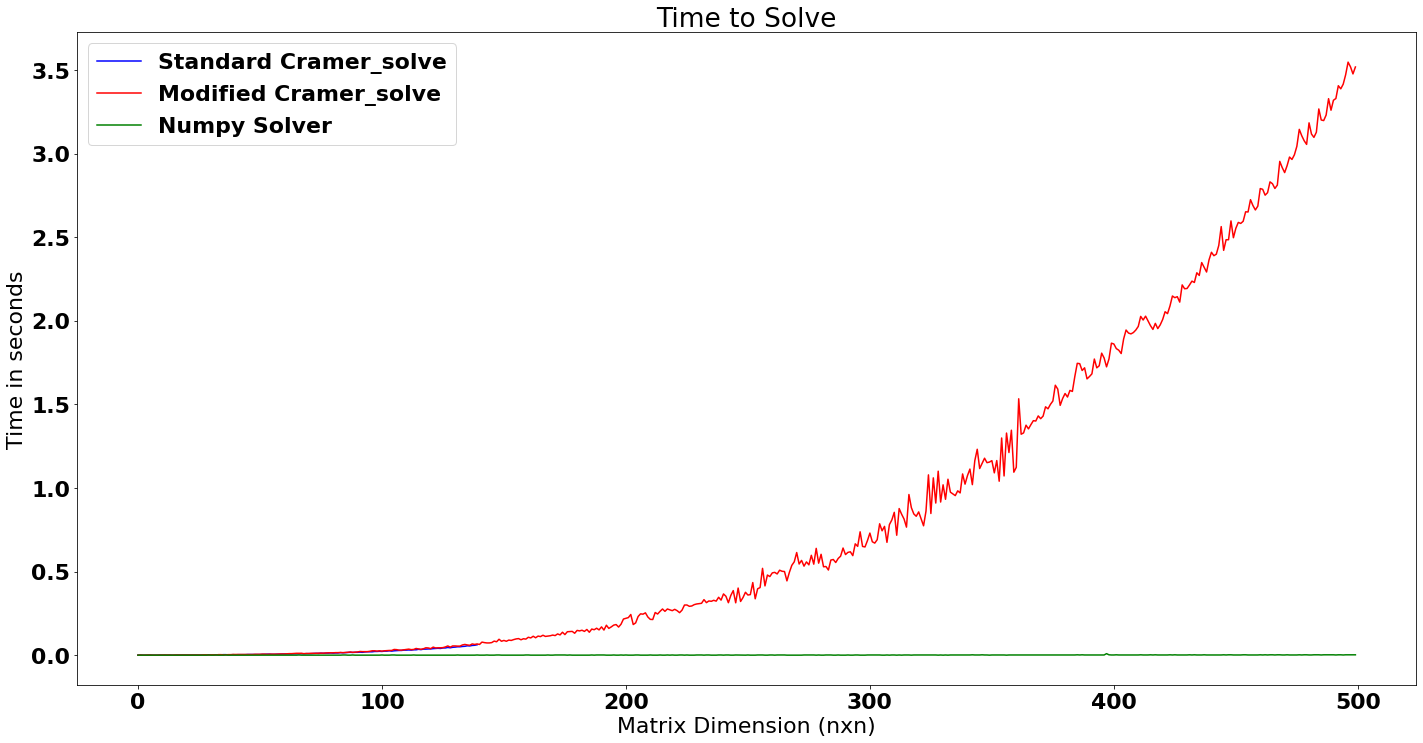
\includegraphics[width=0.8\linewidth]{timer}
\\Note that the standard solver can only salve matrices up to about $150\time 150$.\\
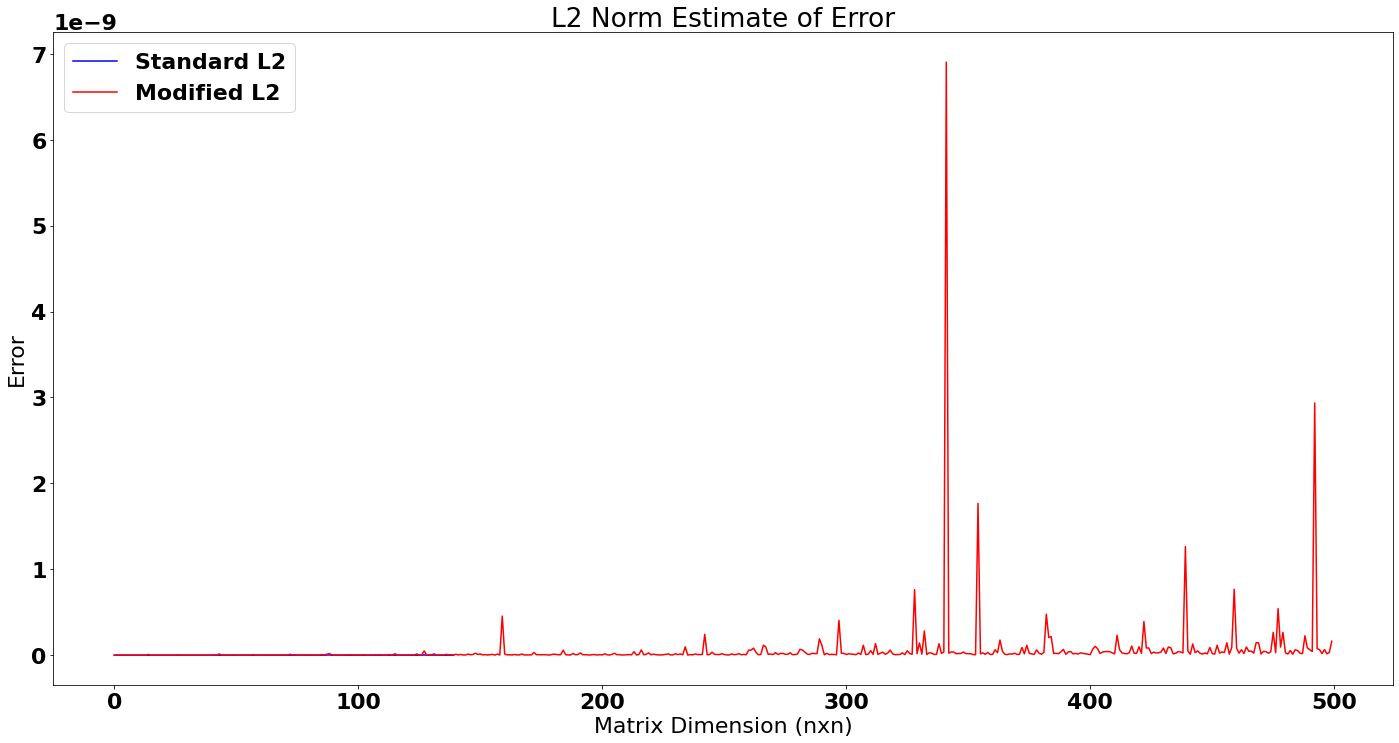
\includegraphics[width=0.8\linewidth]{error}
\\
As we have seen with the gfpp matrix, certain types of matrices can cause both large errors and lengthy execution times. I think that is what occurred at the spikes in the error graph around dimension $350\times 350$.

\section{Thoughts, Opinions, and Future Directions}
I hold the opinion that attempting a more efficient general system of equations solver is not a good use of time. There may be some interesting and large areas of study that involve sparse matrices or specialized solutions. Potential matrices of this type are available through \textit{NLEVP: A Collection of Nonlinear Eigenvalue Problems}, a collection of 52 nonlinear eigenvalue problems in the form of a MATLAB toolbox. (\url{https://github.com/ftisseur/nlevp})

Alternatively, perhaps there is some room for improvement when working with sparse matrices. I did not look closely at sparse matrices to understand the set of algorithms available to solve systems of this type. There are however a number of interesting algorithms that have developed from the human genome project that permit faster classification, ordering or extreme densification of data and may allow for improved results when dealing with sparse matrices.

It is also important to understand how accurate our results need to be. For some systems, dropping half of a properly ordered data set may have minimal impact on the result and would allow for use of additional decomposition methods. Some of this falls into the methods of matrix preconditioning, which is a topic for further review.

\subsection{Classification and Pre-conditioning}
I think that proper, fast, classification of a matrix type would lead to proper selection of a best solution method. Often this is done visually but machine learning has made great strides in classification of images and I think this would be an area for further review.
\\\\
From a cursory reading, I think that pre-conditioning is an approach that is both widely used and potential for further improvement.

\subsection{Is Python the right approach?}
I would argue that python is not really the best language for directly comparing comparing algorithm efficiency. It is fine for the general development of the algorithm but will fail at direct comparison because many of the core underlying algorithms are compiled linked objects. Any code run in the python interpreter will necessarily run slower. If any algorithms are developed, they should be further tested in a compiled language such as Julia.


\section{Resources}
\begin{itemize}
	\item \url{http://web.eecs.utk.edu/~ielhanan/Papers/JDA2011.pdf}
	\item \url{https://www.scirp.org/journal/paperinformation.aspx?paperid=61736}
	\item \url{https://www.math.utah.edu/~gustafso/determinants.pdf}
	\item \url{https://docs.scipy.org/doc/scipy/reference/generated/scipy.linalg.solve.html}
	\item \url{https://www.netlib.org/lapack/explore-html/d7/d3b/group__double_g_esolve_ga5ee879032a8365897c3ba91e3dc8d512.html}
	\item \url{http://www.icl.utk.edu/~mgates3/docs/lapack.html}
	\item \url{https://www.netlib.org/lapack/lug/node71.html} Table 3.13
	\item \url{http://www.ma.man.ac.uk/~higham/mctoolbox/}
	\item \url{https://people.sc.fsu.edu/~jburkardt/py_src/test_mat/test_mat.html}
	\item \url{https://github.com/ftisseur/nlevp}
	\item \url{https://www.bioinformaticsalgorithms.org/}
	\item \url{https://www.netlib.org/linalg/html_templates/node51.html}
	\item \url{https://ieeexplore.ieee.org/document/8742660}
	\item \url{https://www.hindawi.com/journals/isrn/2012/127647/}
\end{itemize}

\begin{align*}
\end{align*}

\begin{align*}
\end{align*}

\begin{lstlisting}[language=Python]
\end{lstlisting}

\noindent\rule{\textwidth}{1pt}
{\footnotesize Copyright (C) 2021 Garold Dalton --- Released under GNU General Public License v3.0}

\cleardoublepage

\end{document}
